\documentclass[a4paper]{article}

% --- Основные пакеты ---
\usepackage{graphicx}     % картинки
\usepackage{geometry}     % поля страницы
\usepackage{hyperref}     % гиперссылки
\usepackage{amsmath}      % математика
\usepackage{amssymb}      % математические символы
\usepackage{float}        % [H] позиционирование фигур
\usepackage[T2A]{fontenc} % кириллица
\usepackage[utf8]{inputenc} % кодировка UTF-8
\usepackage[russian]{babel} % многоязычность
\usepackage{caption}      % настройка подписей

% --- Настройка страницы ---
\geometry{top=1.5cm, bottom=1.5cm, left=3cm, right=1.5cm}

% --- Настройка гиперссылок ---
\hypersetup{
    colorlinks,
    linkcolor=black,
    urlcolor=blue,
    citecolor=black
}

% --- Настройка подписей ---
\renewcommand{\figurename}{Рис.}
\captionsetup{labelsep=period}

\begin{document}

% --- Титульная страница ---
\centering
Министерство науки и высшего образования Российской Федерации\\
Федеральное государственное автономное образовательное учреждение\\
высшего образования\\
«Южно-Уральский государственный университет\\
(национальный исследовательский университет)»\\
Институт естественных и точных наук

\setlength{\parskip}{7.5cm}

Отчет\\
Лабораторная работа №5.\\
Численное дифференцирование.

\setlength{\parskip}{6.5cm}

\raggedleft
\begin{minipage}{0.345\textwidth}
\raggedright
Выполнил: студент группы ЕТ-210\\
Тельнов С.М.\\
Проверил: преподаватель кафедры ВМ\\
Стариков Я.Е.
\end{minipage}

\setlength{\parskip}{6cm}

\centering
Челябинск — 2026

\setlength{\parskip}{0pt plus 1pt}
\newpage

% --- Содержание ---
\centering
\textbf{Краткое содержание}
\begin{itemize}
    \setlength{\parskip}{0.4cm}
    \item \hyperref[sec:theory]{\text{Теоретическая часть} \dotfill \pageref{sec:theory}}
    \item \hyperref[sec:practice]{\text{Практическая часть} \dotfill \pageref{sec:practice}}
    \item \hyperref[sec:conclusion]{\text{Вывод} \dotfill \pageref{sec:conclusion}}
\end{itemize}

\setlength{\parindent}{1.5em}

\raggedright

% --- Теоретическая часть ---
\section*{\centering\fontsize{14pt}{0pt}\selectfont\textbf{Теоретическая часть}\label{sec:theory}}

Целью численного дифференцирования является нахождение приближенного значения производной функции, заданной аналитически или в виде таблицы значений $y_i = f(x_i)$ на равномерной сетке с шагом $h$.

\section*{\fontsize{11pt}{0pt}\selectfont\textbf{Формулы численного дифференцирования}}

Для вычисления первой и второй производных используются конечно-разностные аппроксимации различного порядка точности $O(h^p)$.

Формулы 2-го порядка точности ($p=2$):
\[
y_{i}^{\prime} = \frac{y_{i+1} - y_{i-1}}{2h} + O(h^2)
\]
\[
y_{i}^{\prime\prime} = \frac{y_{i-1} - 2y_i + y_{i+1}}{h^2} + O(h^2)
\]

Формулы 4-го порядка точности ($p=4$):
\[
y_{i}^{\prime} = \frac{y_{i-2} - 8y_{i-1} + 8y_{i+1} - y_{i+2}}{12h} + O(h^4)
\]
\[
y_{i}^{\prime\prime} = \frac{-y_{i-2} + 16y_{i-1} - 30y_i + 16y_{i+1} - y_{i+2}}{12h^2} + O(h^4)
\]

\section*{\fontsize{11pt}{0pt}\selectfont\textbf{Формулы производных через Тейлора}}

Первая производная первого порядка точности (через право)\\
Используем разложение функции в точке $x+h$ в ряд Тейлора:
\[
f(x+h) = f(x) + hf'(x) + O(h^2)
\]
Выразим первую производную $f'(x)$:
\[
f(x+h) - f(x) = hf'(x) + O(h^2)
\]
Разделим обе части на $h$:
\[
f'(x) = \frac{f(x+h) - f(x)}{h} + O(h)
\]

Вторая производная первого порядка точности (через право)\\
Для исключения первой производной нам понадобятся точки $x+h$ и $x+2h$. Запишем их разложения:
\begin{align}
f(x+h)  &= f(x) + hf'(x) + \frac{h^2}{2}f''(x) + O(h^3) \\
f(x+2h) &= f(x) + 2hf'(x) + \frac{4h^2}{2}f''(x) + O(h^3)
\end{align}

Умножим 1-ое уравнение на 2, чтобы выровнять коэффициенты при $f'(x)$:
\[
2f(x+h) = 2f(x) + 2hf'(x) + h^2f''(x) + O(h^3)
\]
Вычтем 2-ое уравнение из 1-го уравнения:
\[
f(x+2h) - 2f(x+h) = -f(x) + h^2f''(x) + \max(O(h^3))
\]
Выразим вторую производную $f''(x)$:
\[
h^2f''(x) = f(x) - 2f(x+h) + f(x+2h) + O(h^3)
\]
Разделим на $h^2$. Получаем правую разностную схему с точностью $O(h)$:
\[
f''(x) = \frac{f(x) - 2f(x+h) + f(x+2h)}{h^2} + O(h)
\]

\section*{\fontsize{11pt}{0pt}\selectfont\textbf{Оптимальный шаг дифференцирования}}

Полная погрешность численного дифференцирования складывается из погрешности метода (усечения) и неустранимой погрешности округления $\epsilon_{\text{окр}}$. При уменьшении шага $h$ погрешность метода убывает, а погрешность округления растет, что обуславливает существование оптимального шага $h_{\text{opt}}$.

Теоретические оценки оптимального шага для различных порядков точности $p$ и производных $m$:

\begin{itemize}
    \item Для первой производной ($m=1$):
    \begin{itemize}
        \item При $p=2$: $h_{opt} = \sqrt[3]{\frac{3\epsilon_{\text{окр}}}{M_{3}}}$
        \item При $p=4$: $h_{opt} = \sqrt[5]{\frac{45\epsilon_{\text{окр}}}{4M_{5}}}$
    \end{itemize}
    \item Для второй производной ($m=2$):
    \begin{itemize}
        \item При $p=2$: $h_{opt} = \sqrt[4]{\frac{48\epsilon_{\text{окр}}}{M_{4}}}$
        \item При $p=4$: $h_{opt} = \sqrt[6]{\frac{240\epsilon_{\text{окр}}}{M_{6}}}$
    \end{itemize}
\end{itemize}

Здесь $\epsilon_{\text{окр}} = \max|y| \cdot \delta_M$ — абсолютная ошибка округления, а $M_k = \max|f^{(k)}(x)|$ — максимальное значение соответствующей производной на интервале.

\newpage

% --- Практическая часть ---
\section*{\centering\fontsize{14pt}{0pt}\selectfont\textbf{Практическая часть}\label{sec:practice}}

\renewcommand{\arraystretch}{1.4}

\section*{\fontsize{11pt}{0pt}\selectfont\textbf{Задание 1}}

\textbf{Задание 1.1.} График исходной функции варианта 10:
\begin{figure}[H]
    \centering
    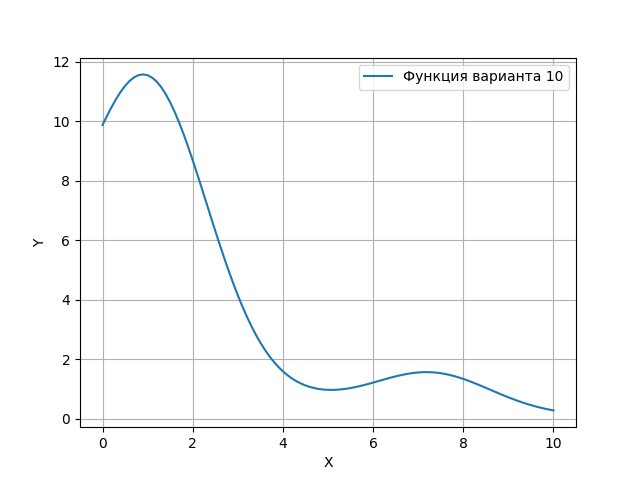
\includegraphics[width=0.75\linewidth]{../pictures/figure_1_1.png}
    \caption{Исходная функция варианта 10.}
\end{figure}

\textbf{Задание 1.2.} 
График 1-ой и 2-ой производной 2-го и 4-го порядка точности соответственно:
\begin{figure}[H]
    \centering
    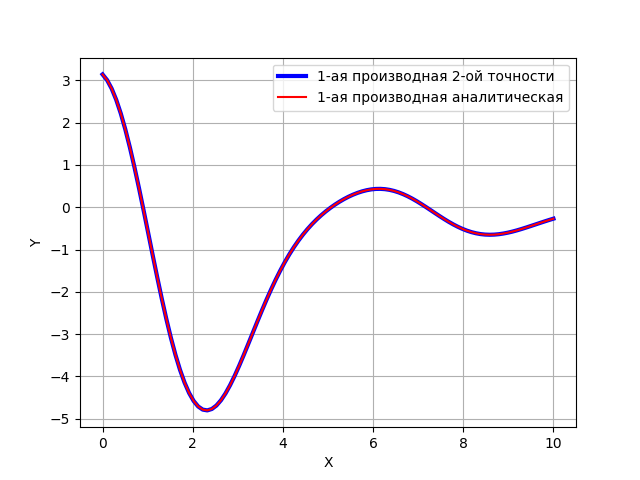
\includegraphics[width=0.75\linewidth]{../pictures/figure_1_2_1.png}
    \caption{1-ая производная 2-го порядка точности.}
\end{figure}
\begin{figure}[H]
    \centering
    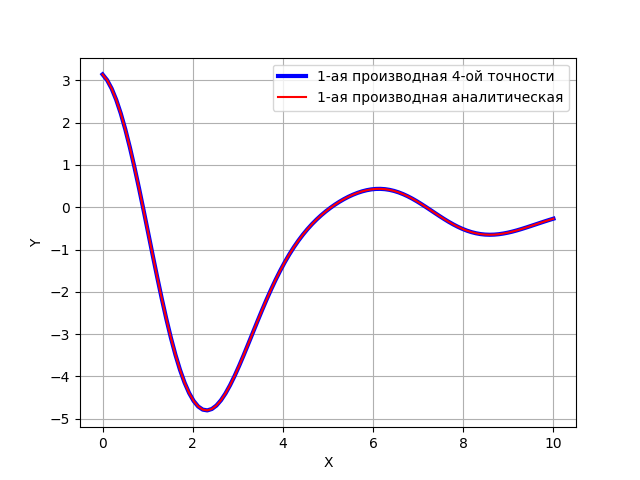
\includegraphics[width=0.75\linewidth]{../pictures/figure_1_2_3.png}
    \caption{1-ая производная 4-го порядка точности.}
\end{figure}
\begin{figure}[H]
    \centering
    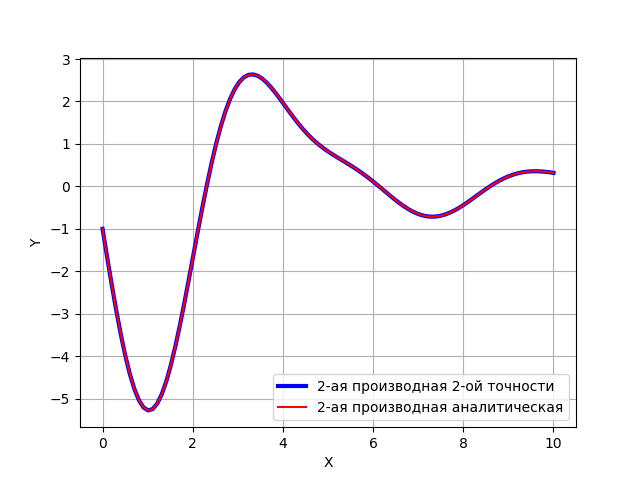
\includegraphics[width=0.75\linewidth]{../pictures/figure_1_2_2.png}
    \caption{2-ая производная 2-го порядка точности.}
\end{figure}
\begin{figure}[H]
    \centering
    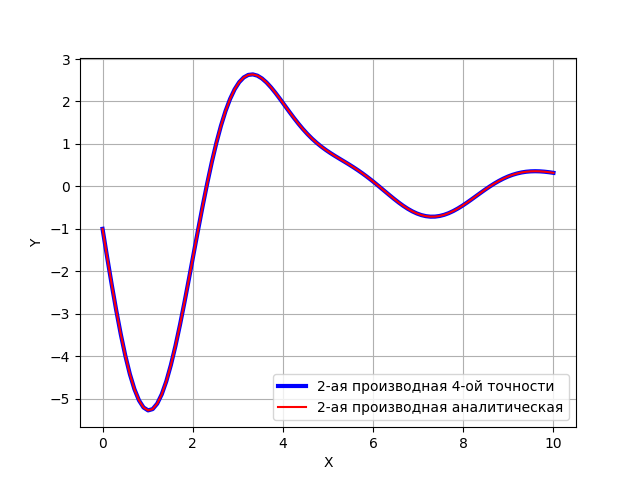
\includegraphics[width=0.75\linewidth]{../pictures/figure_1_2_4.png}
    \caption{2-ая производная 4-го порядка точности.}
\end{figure}

График 1-ой и 2-ой правой производной 2-го порядка полученных из формул Тейлора:
\begin{figure}[H]
    \centering
    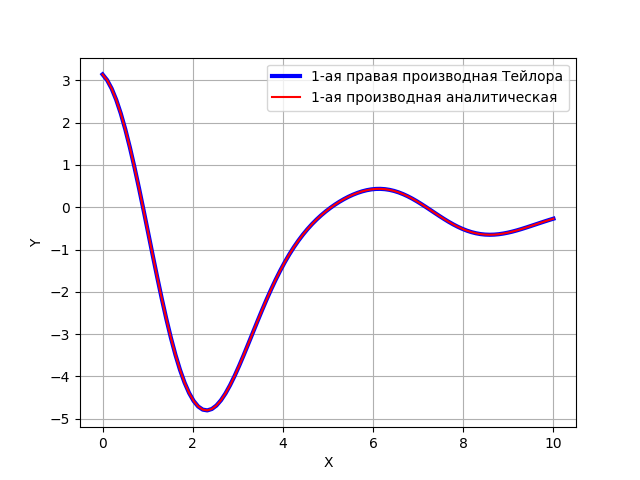
\includegraphics[width=0.75\linewidth]{../pictures/figure_1_2_Teilor_1.png}
    \caption{1-ая правая производная по Тейлору.}
\end{figure}
\begin{figure}[H]
    \centering
    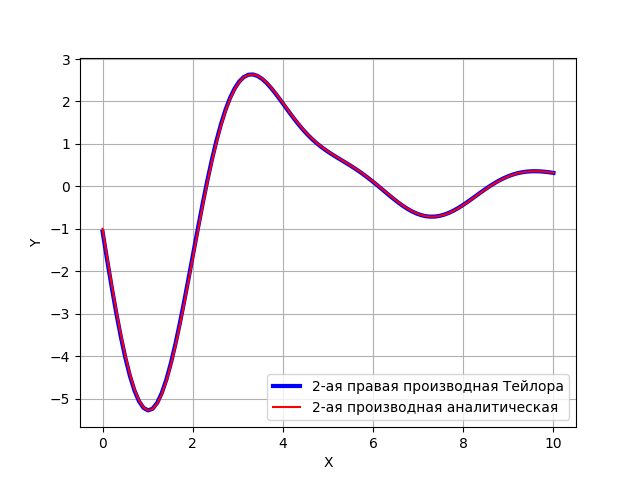
\includegraphics[width=0.75\linewidth]{../pictures/figure_1_2_Teilor_2.png}
    \caption{2-ая правая производная по Тейлору.}
\end{figure}

\textbf{Задание 1.3.} 
График расхождения 1-ой и 2-ой производной 2-го и 4-го порядка точности с аналитическими производными соответственно:
\begin{figure}[H]
    \centering
    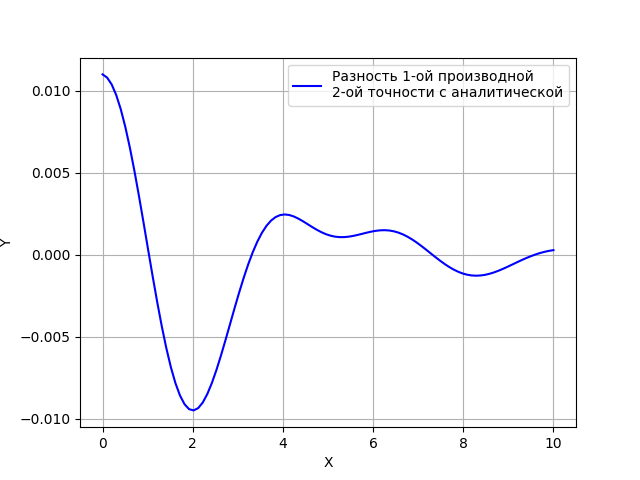
\includegraphics[width=0.75\linewidth]{../pictures/figure_1_3_1.png}
    \caption{1-ая производная 2-го порядка точности.}
\end{figure}
\begin{figure}[H]
    \centering
    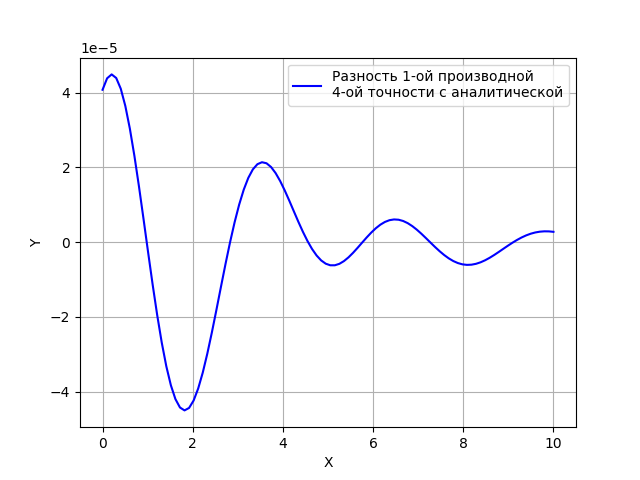
\includegraphics[width=0.75\linewidth]{../pictures/figure_1_3_3.png}
    \caption{1-ая производная 4-го порядка точности.}
\end{figure}
\begin{figure}[H]
    \centering
    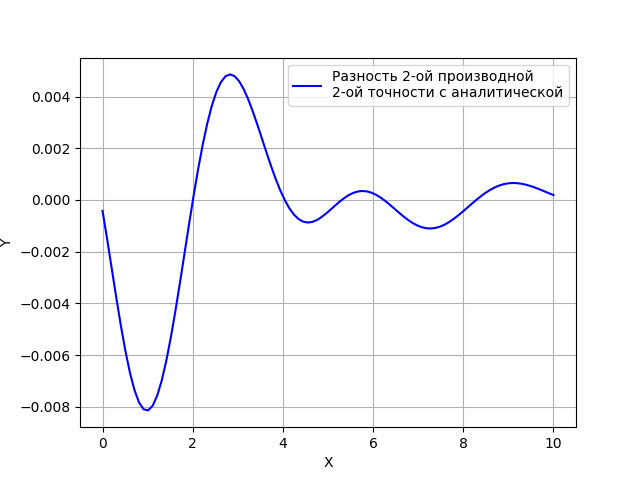
\includegraphics[width=0.75\linewidth]{../pictures/figure_1_3_2.png}
    \caption{2-ая производная 2-го порядка точности.}
\end{figure}
\begin{figure}[H]
    \centering
    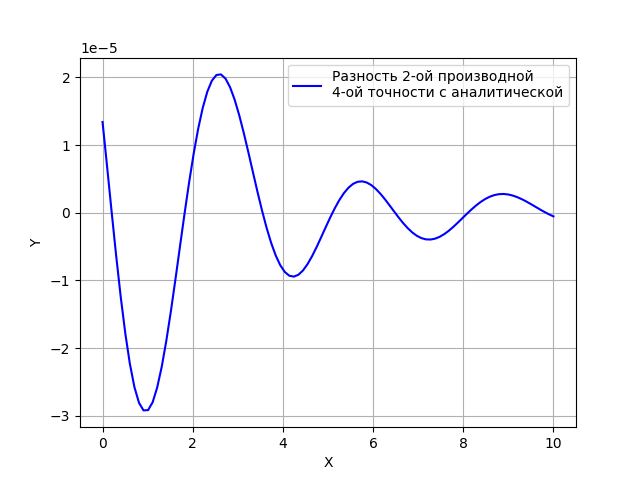
\includegraphics[width=0.75\linewidth]{../pictures/figure_1_3_4.png}
    \caption{2-ая производная 4-го порядка точности.}
\end{figure}

График расхождения 1-ой и 2-ой правой производной 2-го порядка полученных из формул Тейлора с аналитическими производными:
\begin{figure}[H]
    \centering
    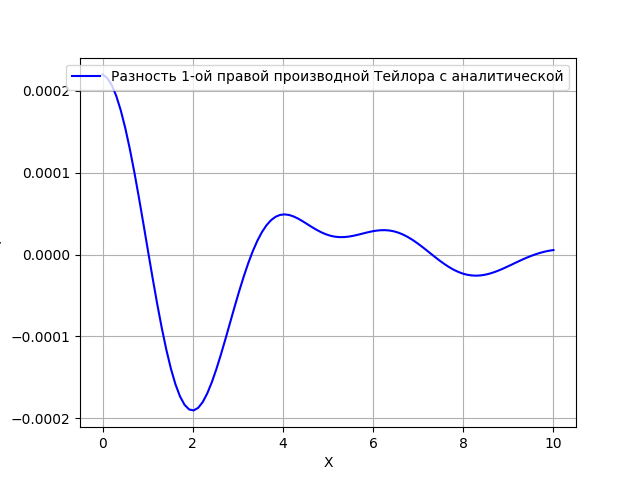
\includegraphics[width=0.75\linewidth]{../pictures/figure_1_3_Teilor_1.png}
    \caption{1-ая правая производная по Тейлору.}
\end{figure}
\begin{figure}[H]
    \centering
    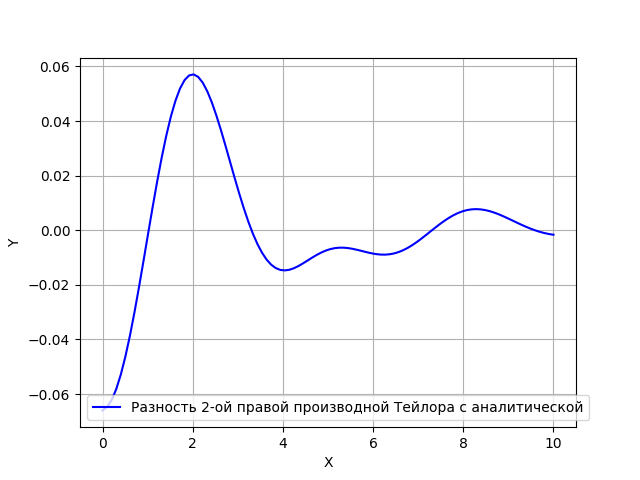
\includegraphics[width=0.75\linewidth]{../pictures/figure_1_3_Teilor_2.png}
    \caption{2-ая правая производная по Тейлору.}
\end{figure}

\textbf{Задание 1.4.} 
Метод подбора шага, точность рассчитывалась как среднее значение модуля расхождения.
Графики ошибки в зависимости от шага в логарифмических осях:
\begin{figure}[H]
    \centering
    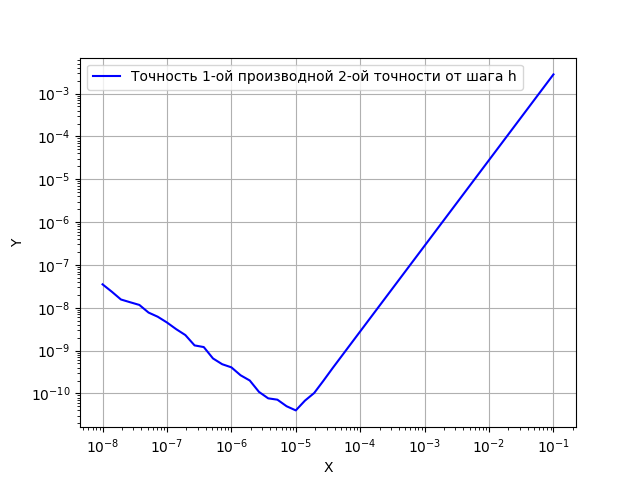
\includegraphics[width=0.75\linewidth]{../pictures/figure_1_4_1.png}
    \caption{1-ая производная 2-го порядка точности.}
\end{figure}
\begin{figure}[H]
    \centering
    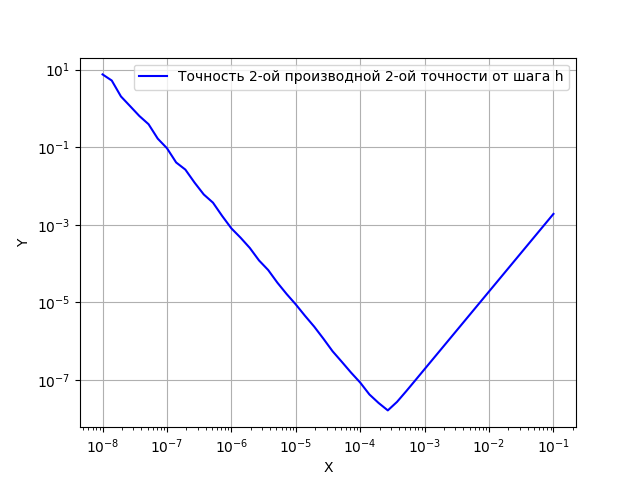
\includegraphics[width=0.75\linewidth]{../pictures/figure_1_4_2.png}
    \caption{2-ая производная 2-го порядка точности.}
\end{figure}
\begin{figure}[H]
    \centering
    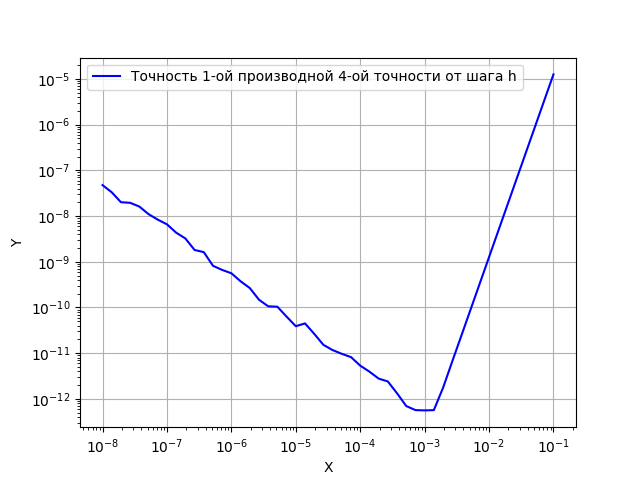
\includegraphics[width=0.75\linewidth]{../pictures/figure_1_4_3.png}
    \caption{1-ая производная 4-го порядка точности.}
\end{figure}
\begin{figure}[H]
    \centering
    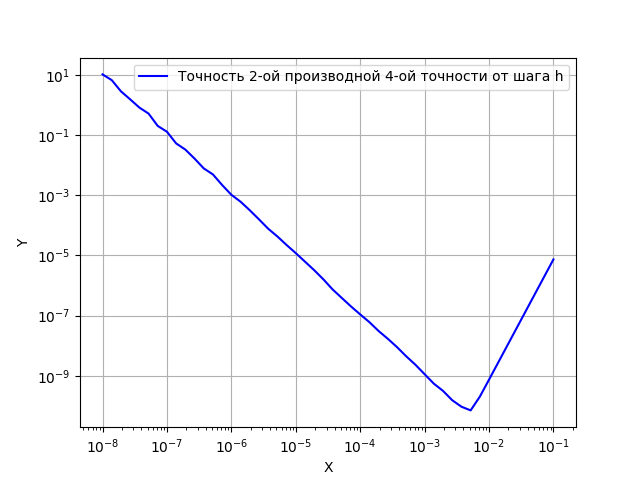
\includegraphics[width=0.75\linewidth]{../pictures/figure_1_4_4.png}
    \caption{2-ая производная 4-го порядка точности.}
\end{figure}
\begin{itemize}
    \item Для 1-ой производной 2-го порядка: $h = 1e-5, \text{accuracy} = 4.014e-11;$
    \item Для 1-ой производной 4-го порядка: $h = 2e-3, \text{accuracy} = 1.65e-8;$
    \item Для 2-ой производной 2-го порядка: $h = 1e-3, \text{accuracy} = 5.6e-13;$
    \item Для 2-ой производной 4-го порядка: $h = 4e-3, \text{accuracy} = 7.029e-11;$
\end{itemize}

Теоретически рассчитанные шаги и их точность при $M^k = 1$:
\begin{itemize}
    \item Для 1-ой производной 2-го порядка: $h = 1.514e-5, \text{accuracy} = 6.729e-11;$
    \item Для 1-ой производной 4-го порядка: $h = 5e-4, \text{accuracy} = 4.574e-8;$
    \item Для 2-ой производной 2-го порядка: $h = 1.7e-3, \text{accuracy} = 1.018e-12;$
    \item Для 2-ой производной 4-го порядка: $h = 8.1e-3, \text{accuracy} = 3.165e-10;$
\end{itemize}

Для всех производных точность производной, полученная методом подбора, выше точности, полученной теоретически.

\section*{\fontsize{11pt}{0pt}\selectfont\textbf{Задание 2}}

\textbf{Задание 2.2.} 
Результат построения интерполяционного полинома и исходной функции:
\begin{figure}[H]
    \centering
    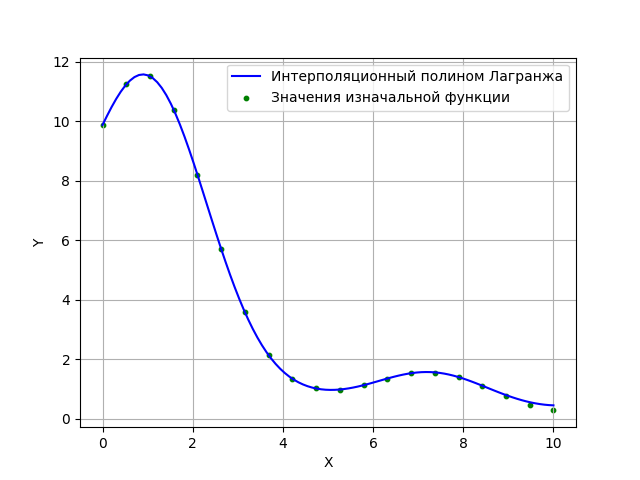
\includegraphics[width=0.75\linewidth]{../pictures/figure_2_2.png}
    \caption{Интерполяционный полином и исходная функция.}
\end{figure}

\textbf{Задание 2.3.} 
Результат построения 1-ой производной и 2-ой производной 2-го порядка точности с их 1-ой и 2-ой аналитическими производными:
\begin{figure}[H]
    \centering
    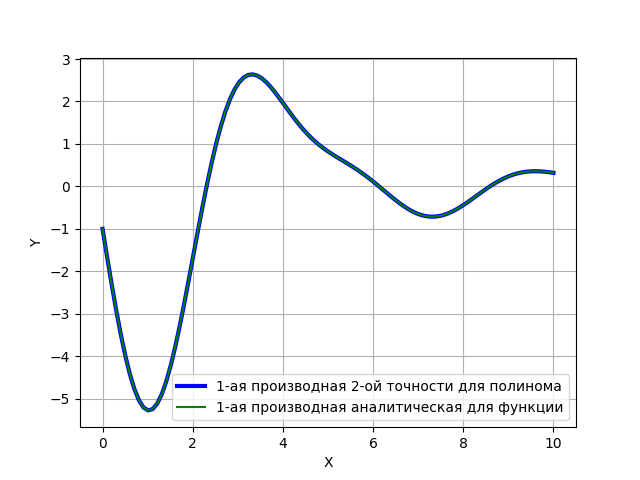
\includegraphics[width=0.75\linewidth]{../pictures/figure_2_3_1.png}
    \caption{Сравнение 1-ых производных.}
\end{figure}
\begin{figure}[H]
    \centering
    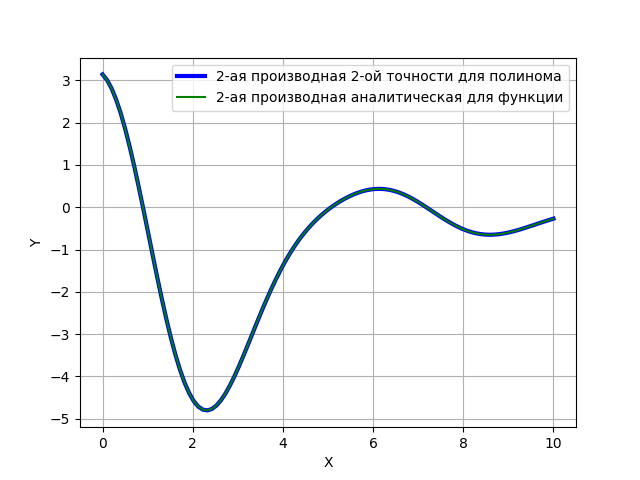
\includegraphics[width=0.75\linewidth]{../pictures/figure_2_3_2.png}
    \caption{Сравнение 2-ых производных.}
\end{figure}

\textbf{Задание 2.4.} 
Результат построения разности 1-ой производной и 2-ой производной 2-го порядка точности с их 1-ой и 2-ой аналитическими производными:
\begin{figure}[H]
    \centering
    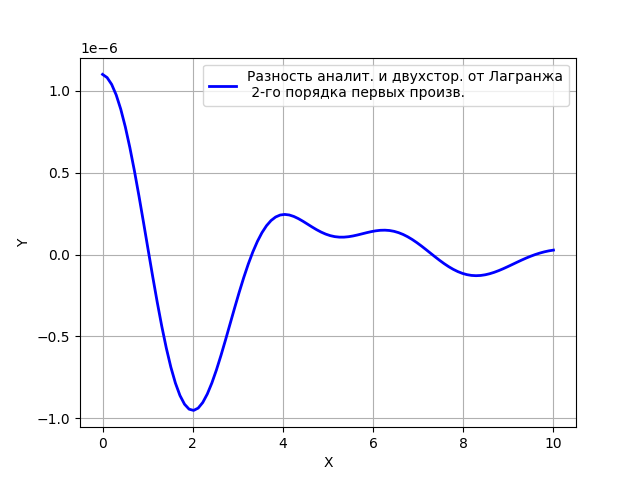
\includegraphics[width=0.75\linewidth]{../pictures/figure_2_4_1.png}
    \caption{Разность 1-ых производных.}
\end{figure}
\begin{figure}[H]
    \centering
    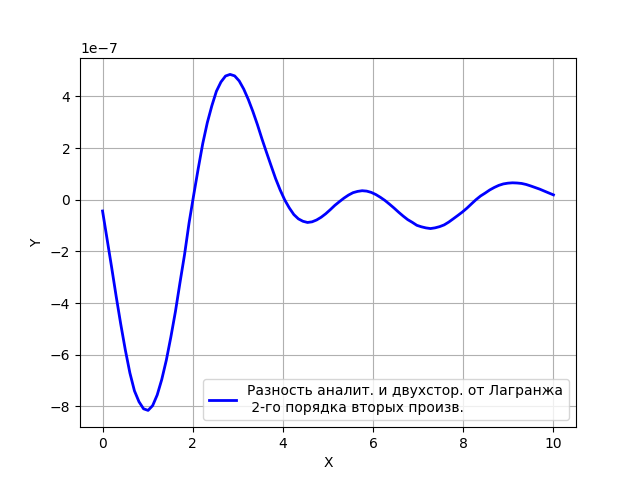
\includegraphics[width=0.75\linewidth]{../pictures/figure_2_4_2.png}
    \caption{Разность 2-ых производных.}
\end{figure}

\newpage

% --- Вывод ---
\section*{\centering\fontsize{14pt}{0pt}\selectfont\textbf{Вывод}\label{sec:conclusion}}

В результате выполнения лабораторной работы были изучены методы численного дифференцирования и проведен сравнительный анализ аппроксимаций различного порядка точности. Сравнение полученных результатов с аналитическим решением показало, что использование формул четвертого порядка обеспечивает значительно меньшую погрешность по сравнению с формулами второго порядка при одинаковом шаге дифференцирования. При анализе влияния величины шага на точность расчетов было подтверждено наличие оптимального значения $h$, при котором суммарная ошибка минимальна. Это обусловлено тем, что при больших значениях шага преобладает погрешность метода, а при критически малых — резко возрастает вычислительная погрешность, вызванная потерей значащих цифр при вычитании близких чисел. Построенные графики расхождения наглядно иллюстрируют эти теоретические положения. Кроме того, применение интерполяционных полиномов для нахождения производных таблично заданных функций подтвердило эффективность сочетания методов аппроксимации с последующим численным дифференцированием, что позволяет сглаживать локальные возмущения в исходных данных и получать устойчивые результаты.

\end{document}
